\chapter{Introduction}

\section{Motivation}
\gls{ic} is a faculty of \gls{kmitl}. 
IC has been up and running well for 6 years.
About 25 employees are working here.
Their main objective is to provide educational services to students. 
Right now, they have a trouble with paper clutter. 
Even though they have organized documents into categories. 
The organization takes countless hours to organize, store, and retrieve documents.
This problem hinders employee's productivity when they need to retrieve many documents. 
Another problem is losing track of document during its workflow execution. 
A workflow is a series of repeatable steps performed in a sequential manner to reach a goal.
Each type of workflow usually associates with a set of actions. 
A person who receive a document will execute some actions depending on their responsibility.
They have to execute them sequentially. 
Some workflows are very complicated and very difficult to keep track of.

IC would like to prevent these problems before it goes out of control. 
Our proposed solution is to manage, store, and retrieve documents digitally using a computer software.
The employee will use less time to search and be less error-prone.
We will create a system that provide ability to search and to track documents.
We are working on \MakeLowercase{\dms}, or so called Monkey Office.
Because we want to provide a system to manage documents within IC.
Once we do, IC can manage and track documents more efficient, thus, increase organization's productivity.

\section{Objective}
% list of our primary objectives
Our primary objectives are
\begin{enumerate}
\item To design a workflow model and to track document's current state during its workflow execution. 
\item To report other related or dependent documents required by its originator.
\item To store and retrieve digital documents corresponding to outgoing or finished workflows from and to IC's server.
\end{enumerate}

\section{Scope}
We are going to develop a web-based application hosted on an IC's server.
Only people within IC and granted external users can access the system.
To be specific, there are 4 types of users.
\begin{enumerate}
\item IC's administrative staffs.
\item KMITL lecturers who is assigned to IC.
\item Students who are currently enrolled in IC, KMITL.
\item External users who is allowed to access the system by IC e.g.\ Alumni students.
\end{enumerate}

Before diving deeper into the scope of this project, we would like to clarify these 2 words---document and workflow---in terms of our project. %transition
Because from now on, we will use these words frequently and we would like readers to interpret them correctly.
%TODO Explain what is a document
Firstly, a document is a record that provides information or served as an evidence.
Pictures and sound can also be considered as a document both in physical and digital form. %TODO cite %TODO cite oxford dict http://goo.gl/Ziutvi and http://goo.gl/5x6EOZ
%TODO Explain what is a workflow
Secondly, a workflow is a sequence of repeatable tasks performed to achieve a single goal. %TODO cite
Each tasks may perform with specific conditions.
A person, machine, group of persons or machines are responsible to carry out the task. %TODO cite http://goo.gl/IayPio
%TODO Explain how workflow and document are related
So, how workflow and document are related together?
In organizations, the goal of the document is get them approved, distributed, or archived.
A document can be an input or end-product of the task.
The task may require a certain document to execute.
Other documents may be produced by the task.

Our primary focus is digital documents produced from tasks in the workflow.
The system has to manage workflows which are created officially by IC and documents produced by tasks.
The system offer document file hosting services to users for reusing them later.
Hosted documents that are not used by the workflow is not in the scope of this project.
Uploaded documents that is not in the system's file hosting service is in the scope if IC requires them in one of the task in workflow.
This thesis conducts only on the following 2 types of documents.
%TODO How these 7 types are related to form, resulting docs, attachments, ...
\begin{enumerate}
\item Electronic form \hfill \\
A formatted document with blank fields that prompts user to fill in.
Forms are created according to IC's work procedure and instruction.
Work procedure provides details on working procedures, departments, or persons who hold responsibilities for documents.
Work instruction indicates employee's roles and responsibilities.
IC defines non-filled form as ''Form'' and already filled form as ''Record''.
By the time of writing, this project conduct with 3 sub-types forms.
\begin{enumerate}
\item Absence form \hfill \\
For IC's employee and students to take days off due to personal or business reasons.
\item Student internship form \hfill \\
For IC students who is above Year 2 to gain work experience in software industry during a summer semester.
\item Conference outside KMITL form \hfill \\
For lecturers to request going to a conference outside KMITL.
\end{enumerate}
Because all of these forms are in paper-based format, we have to convert them into the electronic form.
Meaning that a system displays the form on a computer screen waiting for a user to fill in required blank fields.
\item External document \hfill \\
Documents received from other individuals or departments in order to proceed some tasks in a workflow.
If received document is in paper form, it has to be scanned by a scanner first.
The task includes these documents as attachments.
\end{enumerate}

\section{Project plan}
The project starts at August 18th, 2015.
We expect to deliver it on March 25th, 2016.
For our project planing, we divide our work into 4 phases.
%TODO descibe them
\begin{enumerate}
\item Plan and research (18/08/15 -- 30/10/15) \hfill \\
The first phase was to gather user's requirements by interviewing.
We interviewed with IC's vice dean because he is a client who came up with this project.
Then, we moved on to interviewing IC's employees asking about document related problem they encountered.
Next, we discussed about software tools that solve the problem.
\item Design and architecture (29/09/15 -- 23/11/15) \hfill \\
On the second phase, we designed the software architecture.
The architecture is the core of how software must behave, also to get an overview of system interaction.
Then, we designed a \gls{gui} of this system.
\item System implementation (7/12/15 -- 22/02/16) \hfill \\
This phase began writing source codes based on user requirements, designed architecture, and technical specification.
Later on, we connected each system's components together.
\item Testing (19/02/16 -- 07/03/16) \hfill \\
This phase ensured that systems ran correctly with user and system requirements.
We also conducted user acceptance testing.
Then, We evaluated testing result.
If the result were satisfying, we would deploy the system to IC's server.
\end{enumerate}

\begin{landscape}
\begin{figure}
\centering
\caption{Project's schedule shown as Gantt chart}
\label{fig:project-schedule}
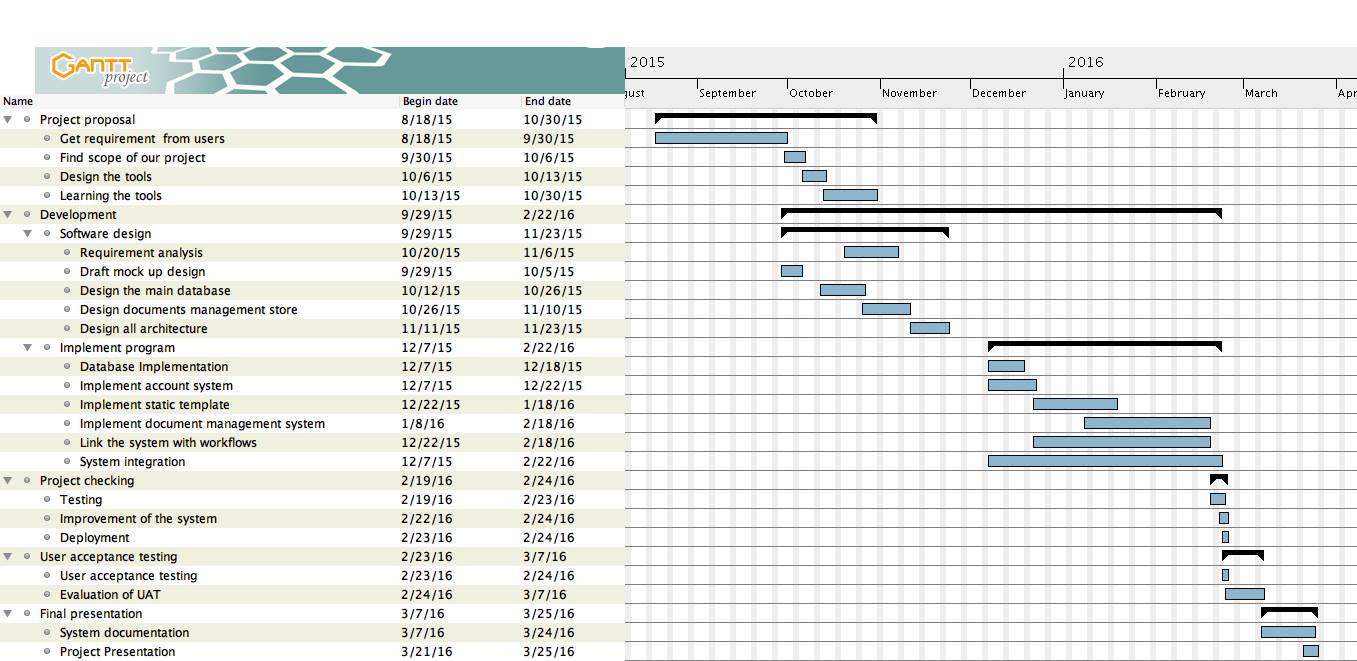
\includegraphics[scale=0.45]{res/project_plan}
\end{figure}
\end{landscape}